\documentclass[../../main.tex]{subfiles}

\begin{document}

We will use 1D datasets to firstly optimize the hyperparameters of the TNP models and use this to compare the performance of the TNP and ConvNP models. The metric used to compare the models is the validation loss of the models on unseen data. Furthermore, we will look at the plots of the predictions to observe the behavior of the models especially in the regions outside the training data.


\section{Datasets}

\subsection{Gaussian Process}
\label{sec:1d-gp-dataset}

We will use samples from a Gaussian Process to generate the data. The aim will be for our model to learn the underlying function of the Gaussian Process and recover the underlying process. The Gaussian Process is defined as:

\begin{equation}
	f(x) \sim \mathcal{GP}(0, k(x, x'))
\end{equation}

Where we use the squared exponential kernel:

\begin{equation}
	k(x, x') = \exp\left(-\frac{(x - x')^2}{2l^2}\right)
\end{equation}

With length scales being sampled from a uniform distribution $l \sim \mathcal{U}(\log(-0.101), \log(0.101))$. We choose to sample $N_c$ context points from the Gaussian Process and use these as the training data for our models. We then sample $N_t$ target points from the Gaussian Process and use these as the validation data for our models. Depending on the specific task we will either fix or vary the number of context points $N_c$ and target points $N_t$.


\subsection{Sawtooth}
\label{sec:1d-sawtooth-dataset}

Whilst the GP is useful for testing the models on a smooth function, we also want to test the models on a more complex function, particularly one with discontinuities. We will use the sawtooth function for this purpose. The sawtooth function with period $T$ is defined as:

\begin{equation}
	f(x) = x - T \left\lfloor \frac{x}{T} \right\rfloor + n
\end{equation}

Where $n$ is some random noise which is sampled from a normal distribution $n \sim \mathcal{N}(0, 0.1)$.
We will sample $N_c$ context points from the sawtooth function and use these as the training data for our models. We then sample $N_t$ target points from the sawtooth function and use these as the validation data for our models. Depending on the specific task we will either fix or vary the number of context points $N_c$ and target points $N_t$.


\section{Relative Attention Function}

As mentioned in \autoref{sec:tetnp} we need to pass the matrix of differences ($\bm{\Delta}$) between $x$ values through a function $F$ to apply non-linearities to the differences acting as hyperparameter of our mode. We will investigate using a simple linear function with no bias and gradient 1 (`identity') as a baseline. For non-linear functions, we will consider using a Gaussian Radial Basis Function (RBF) and a Multi-Layer Perceptron (MLP). The functions are defined below:

\begin{align}
	F_{\text{identity}}(\Delta) &= \Delta&
	F_{\text{RBF}}(\Delta) &= \exp\left(-\frac{\Delta^2}{2\sigma^2}\right)&
	F_{\text{MLP}}(\Delta) &= \text{MLP}(\Delta)
\end{align}

Where $\sigma$ is a hyperparameter of the RBF function and $\text{MLP}(\Delta)$ is a 2-layer MLP with ReLU activation functions.

\begin{figure}[H]
	\centering
	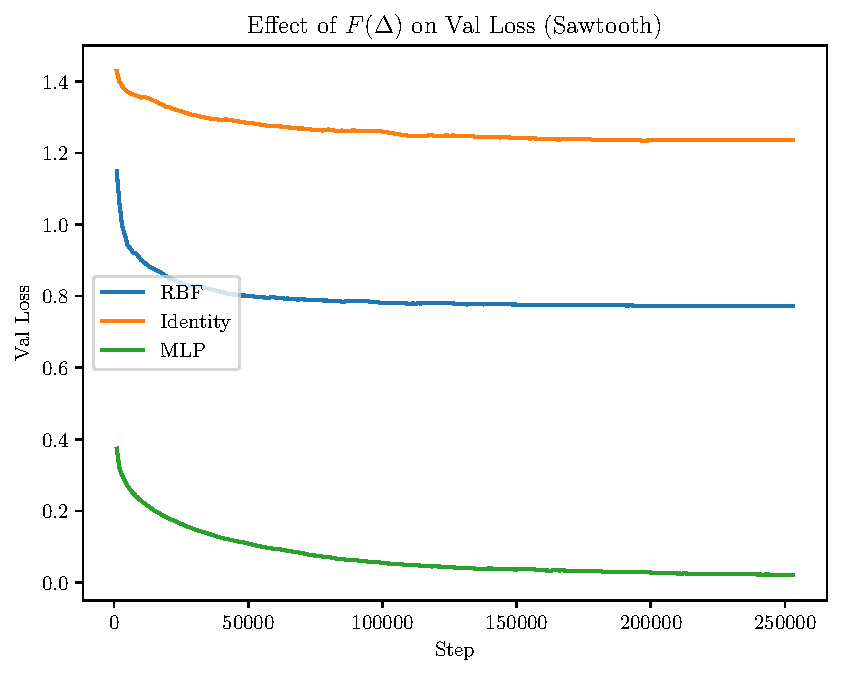
\includegraphics[width=0.6\linewidth]{./F-on-loss.pdf}
	\caption{Relative Attention Functions on Validation Loss for the TETNP on the 1D Sawtooth Dataset. Lower validation loss is better.}
	\label{fig:relative-attn-func-1d}
\end{figure}

\autoref{fig:relative-attn-func-1d} shows the validation loss curves for the TNP with different relative attention functions. We can see that the MLP function performs significantly better than the other two functions. This is likely due to the MLP being able to \textbf{learn} whilst the other two functions are fixed. We can also see that the RBF function performs better than the identify function since the effect of adding the raw difference affects the dot product of the attention mechanism. So we can conclude that the MLP function is the best function out of three we considered. The computational cost of using the MLP function is also not significantly higher than the other two functions, since the MLP is very small.



\section{Optimizing Hyperparameters}

The multi-headed attention mechanism in the Transformer Encoder has three hyperparameters that we will investigate. These are
the token embedding dimension of the data ($D_{em}$), the number of attention heads ($N_h$) and the embedding dimension of the attention heads ($D_h$). We will investigate how changing these hyperparameters affects the performance of the model. To gauge the effect of these hyperparameters, we use a 1 million parameter model and reduce the value of one of the hyperparameters and see the effect on the validation loss. This process is repeated for the other hyperparameters to see which hyperparameters have the most effect on the validation loss. 



\begin{figure}[H]
	\centering
	\subfloat[Token Embedding Dimension]{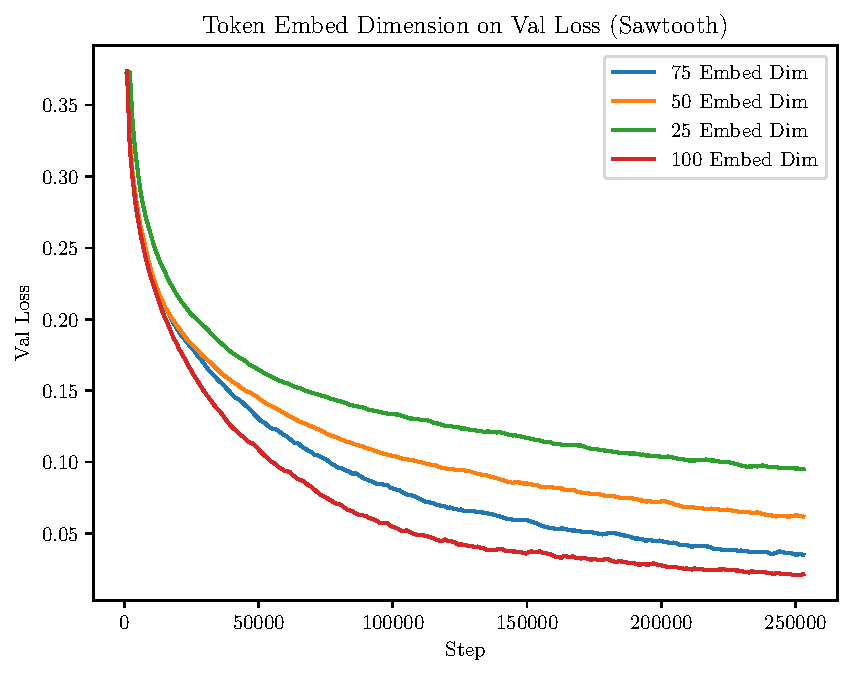
\includegraphics[width=0.5\linewidth]{./embed-dim-on-loss.pdf}\label{fig:hyperparam-optimization-token}}
	\subfloat[Number of Heads]{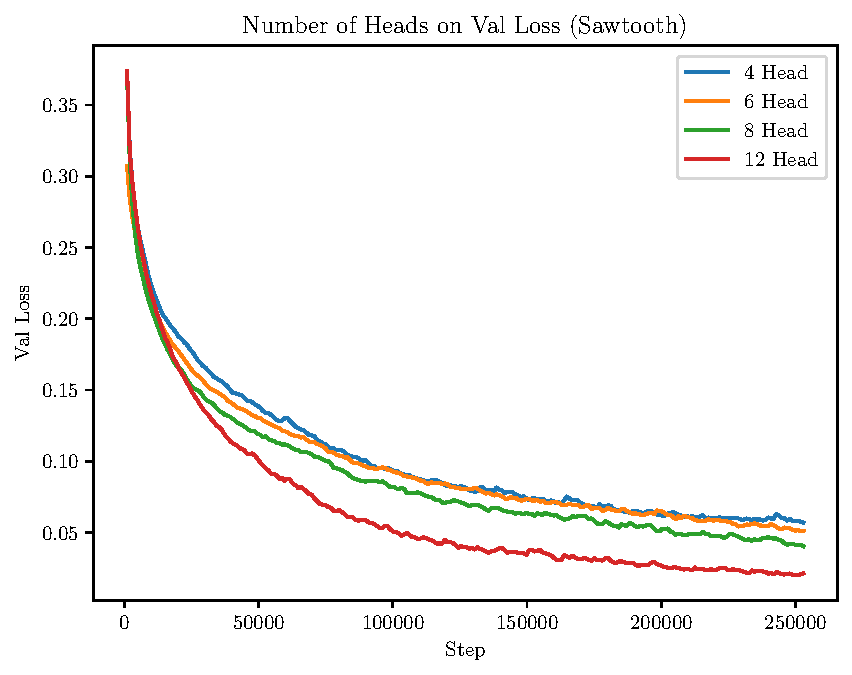
\includegraphics[width=0.5\linewidth]{./head-count-on-loss.pdf}\label{fig:hyperparam-optimization-num}}\\
	\subfloat[Head Embedding Dimension]{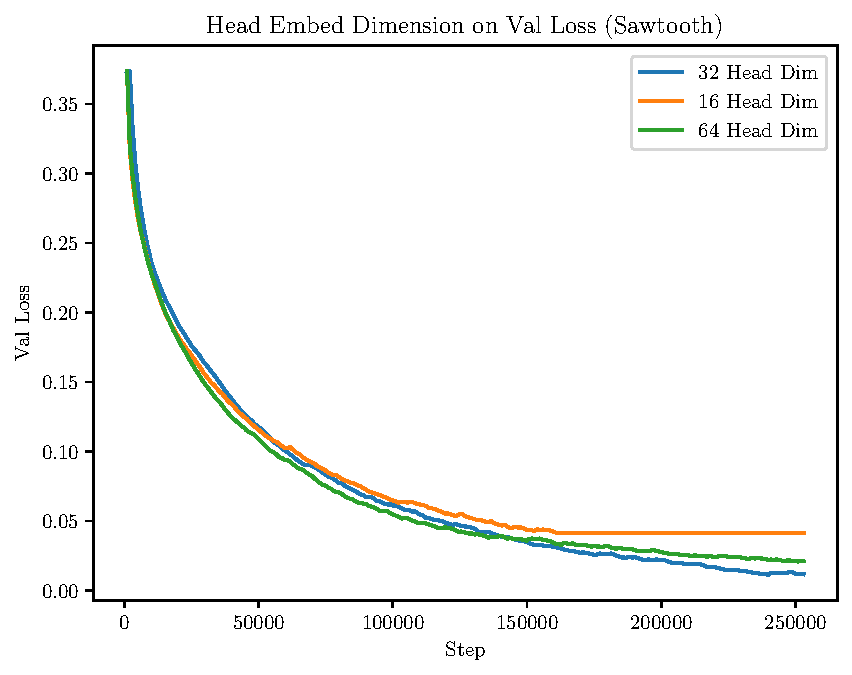
\includegraphics[width=0.5\linewidth]{./head-dim-on-loss.pdf}\label{fig:hyperparam-optimization-head}}
	\caption{Hyperparameter Selection}
	\label{fig:hyperparam-optimization}
\end{figure}

From \autoref{fig:hyperparam-optimization} it is clear that reducing the token embedding dimension has a significant effect on the validation loss, with the number of heads making a smaller difference and the head embedding dimension making very little difference. This highlights the importance of the token embedding dimension even when using low one-dimensional data as the input data (in this case sawtooth function). Furthermore, the head embedding dimension has very little effect on the validation loss, so we can set this to a small value to reduce the number of parameters in the model and distribute the parameters to the other hyperparameters. Using this knowledge, we will now investigate how to select the hyperparameters using a \emph{constant parameter budget} of 1 million parameters. 

% 1m.jpg

\FloatBarrier
\begin{figure}[ht!]
	\centering
	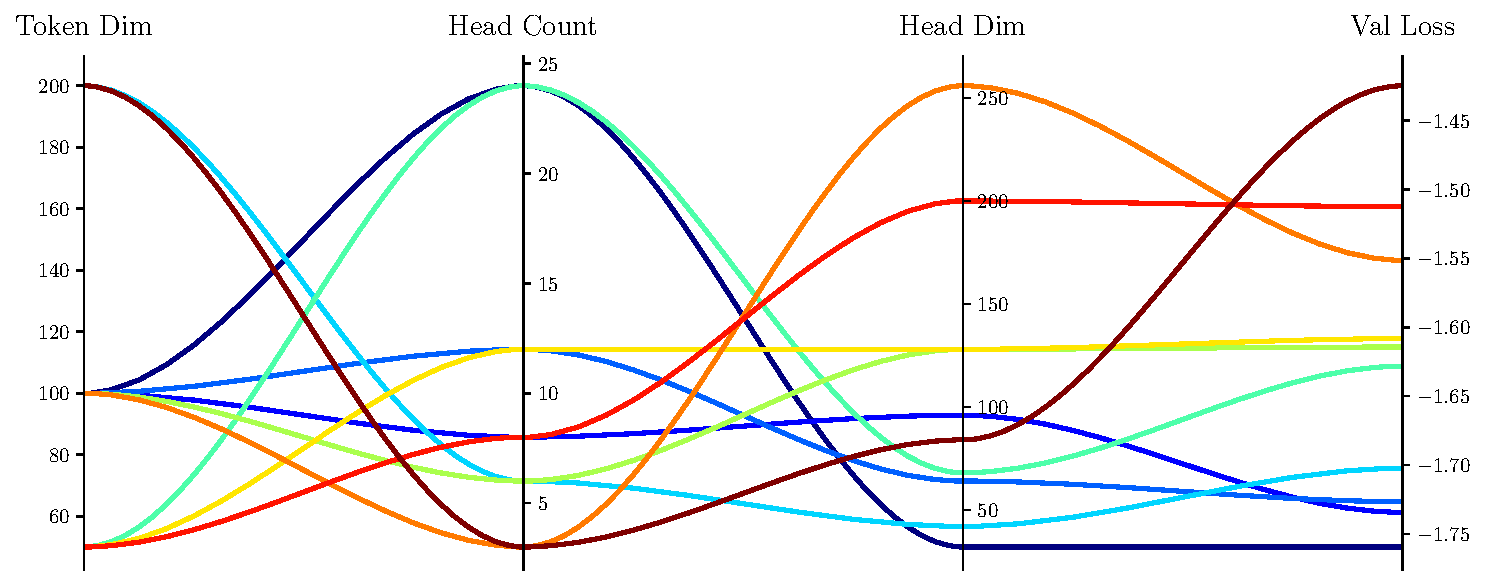
\includegraphics[width=0.9\linewidth]{./model-comparsion-1d.pdf}
	\caption{Constant Parameter Budget Hyperparameter Selection}
	\label{fig:1m-parameter-budget}
\end{figure}
\FloatBarrier

\autoref{fig:1m-parameter-budget} shows a parallel coordinates plot of the validation loss for different hyperparameter configurations, where dark blue is the best and dark red is the worst. We can see that the model that performs the best has a very high token embedding dimension, high headcount and low head embedding dimension, which is consistent with the previous results. We can also see that if we go too high in the token embedding dimension (200), the model performs worse as we have to sacrifice the number of heads in the transformer. These results give us a set of best practices for selecting hyperparameters for the TNP: high token embedding dimension, high number of heads and low head embedding dimension.





\section{TNP vs ConvNP}

% \subsection{Model Fits}

Finally, using our `best' TNP model, we will compare the performance of the ConvNP and TNP on fitting sawtooth and GP (using EQ Kernel) data using 1 million parameters. 

% result.png

\begin{figure}[H]
	\centering
	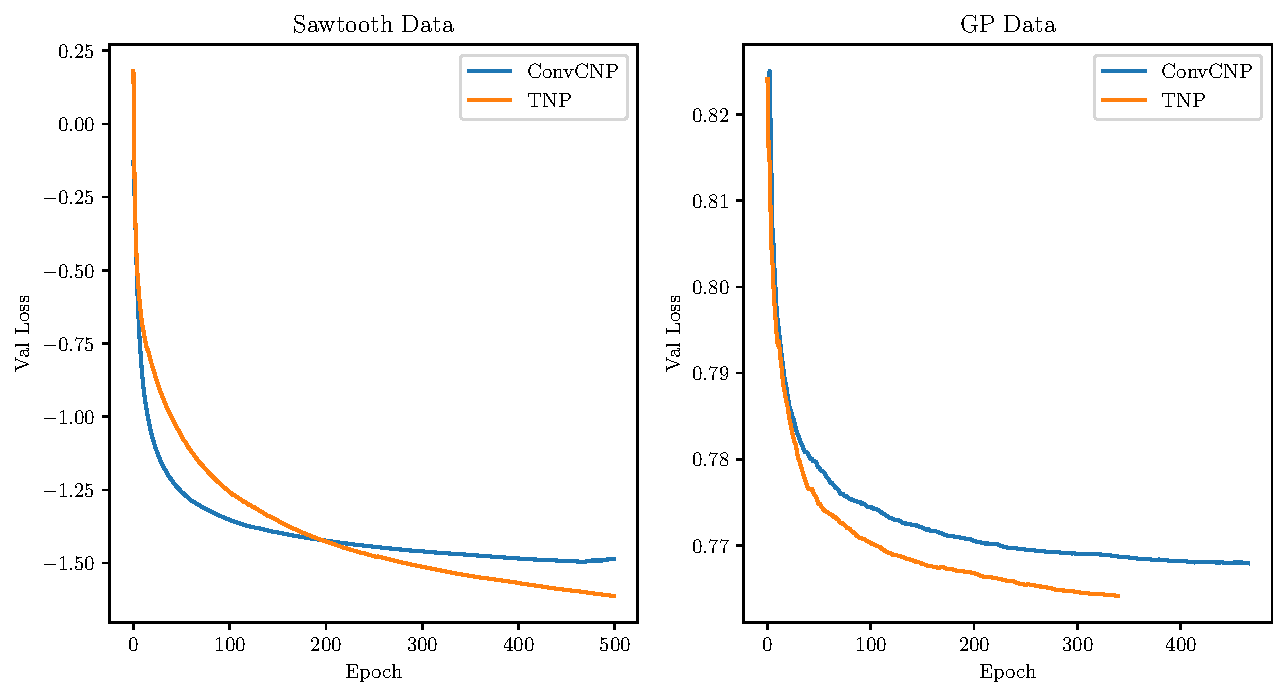
\includegraphics[width=0.5\linewidth]{./convcnp-vs-tetnp-saw-gp.pdf}
	\caption{ConvNP vs TNP on Sawtooth and GP Data}
	\label{fig:conv-tnp-1d-result}
\end{figure}

\autoref{fig:conv-tnp-1d-result} shows the validation loss curves for the ConvNP and TNP on sawtooth and GP data. We can see that the validation loss for the TNP is lower than the ConvNP for both datasets which is very promising and indicates the TNP is a better model than the ConvNP. 


\begin{figure}[H]
	\centering
	\subfloat[TNP]{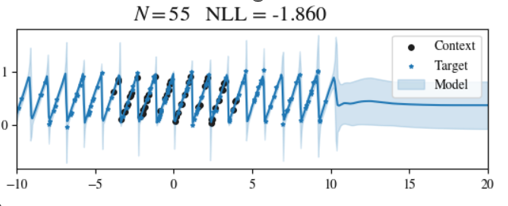
\includegraphics[width=0.47\linewidth]{./tnp_saw.png}\label{fig:1d-sawtooth-comparisons-tnp_saw}}
	\qquad
	\subfloat[ConvNP]{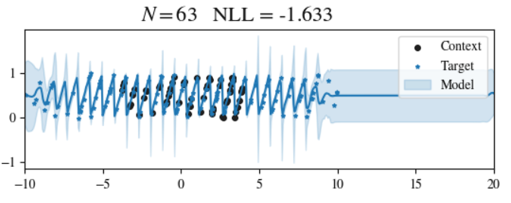
\includegraphics[width=0.47\linewidth]{./convnp_saw.png}\label{fig:1d-sawtooth-comparisons-convnp_saw}}
	\caption{ConvNP vs TNP on Sawtooth Data. The context set inputs are between [-4, 4] and the target set inputs are between [-10, 10] which extends beyond the context set to test the models' extrapolation capabilities.} 
	\label{fig:1d-sawtooth-comparisons}
\end{figure}

Inspecting the model fits on sawtooth data \autoref{fig:1d-sawtooth-comparisons}, we observe that the TNP can extrapolate the structure of the sawtooth function beyond the range of the context set (black points) whilst the ConvNP performs decently but fails to retain the structure as well as the TNP, since the amplitude of the sawtooth reduces the further away from the context set. Hence we can conclude that the TNP can better understand the structure of the data than the ConvNP.

\subsection{Computational Complexity}

\begin{table}[htpb!]
	\centering
	\begin{tabular}{@{}llcc@{}}
	\toprule
	$N_c$ & $N_t$ & ConvNP Memory (MB) & TETNP Memory (MB) \\ \midrule
	10    & 10    & 18                 & 13                \\
	100   & 10    & 16                 & 18                \\
	1000  & 10    & 16                 & 339               \\
	5000  & 10    & 124                & 9357              \\ \midrule
	10    & 1000  & 36                 & 399               \\
	100   & 1000  & 36                 & 469               \\
	1000  & 1000  & 36                 & 1510              \\
	5000  & 1000  & 124                & 13480             \\ \bottomrule
	\end{tabular}
	\caption{Memory Usage in inference of the ConvNP and TETNP on 1D data using $N_c$ context points and $N_t$ target points.}
	\label{tab:memory-usage-comparison}
\end{table}

\autoref{tab:memory-usage-comparison} shows that the TETNP uses drastically more memory than the ConvNP for the same number of context and target points. This is due to the quadratic complexity of the TETNP which scales with $\mathcal{O}(N_c^2 + N_cN_t)$ compared to the linear complexity of the ConvNP which scales with $\mathcal{O}(N_cD_x^3 + N_tD_x)$. Whilst on the 1D dataset the ConvNP is more memory efficient, the TETNPs complexity does not scale with the number of dimensions of the data, whilst the ConvNP \emph{scales cubically with the number of dimensions}. This may suggest that the TETNP is more suitable for high-dimensional data than the ConvNP since the TETNP has a fixed memory cost per dimension. We will investigate this in the next chapter on 2D datasets to see if the discrepancy in memory usage is still present.

\ifSubfilesClassLoaded{%
    \printbibliography{}
}{} 


\end{document}